%   Titre de la sous section
\section{Ton premier programme avec \mb}

%   logo mb  dans la table des matières
\logo{mb}

\pagestyle{mb}

\subsection{Description}

\subsubsection{Objectif}

%   bloc de formule
%   sans titre et fond bleu cyan
\begin{formule}
Une minute top chrono !\\
Il vous faudra un peu plus de temps (mais à peine) pour réaliser ce premier programme, qui vous permettra de simuler un sablier. Ou alors d'égréner le temps qui passe durant ce cours interminable.

Voilà de bons prétextes pour découvrir les possibilités offertes par  \mb !
\end{formule}


\subsubsection{Intérêt}

%liste d'arguments
\begin{description}
    \item [découvrir l'interface de programmation] et élaborer son premier programme;
    \item [découvrir quelques fonctions] pour avoir envie d'en savoir plus;
    \item [programmer un objet] très facilement.
\end{description}


\subsubsection{Matériel}
\begin{itemize}
%   matériel pour micro:bit
    \item 1 $\times$ \matosMb (mais un accès internet peut suffir)
%   site pour micro:bit
    \item 1 $\times$ accès internet : IDE programmation par bloc \url{http://makecode.microbit.org/}
\end{itemize}


\subsubsection{Pour commencer}

\begin{itemize}
  \item Se munir d'un \mb et de son cable usb;
  \item Brancher un \mb sur l'ordinateur;
  \item Ouvrir un navigateur internet récent et aller sur la page citée au-dessus.
  \item Cliquer sur 
\includegraphics[width=0.1\linewidth]{res/mb-makecode_1erProg_nouvProj.png}
\end{itemize}


\subsubsection{Prise en main}

\begin{minipage}[t]{0.75\linewidth}
Lors du démarrage d'un nouveau projet, l'interface place par défaut dans l'espace de travail les blocs \emph{au démarrage} et \emph{toujours}; or nous n'avons pas besoin de ce dernier pour notre projet. Pour s'en débarrasser il suffit de le saisir et le lâcher vers la gauche, au dessus du menu des catégories.
\end{minipage}
%   petit "ressort"
%   pour centrer les 2 colonnes
\hfill
%   colonne de droite
\begin{minipage}[t]{0.25\linewidth}~\\
  \vspace{-5mm}
  \begin{center}
    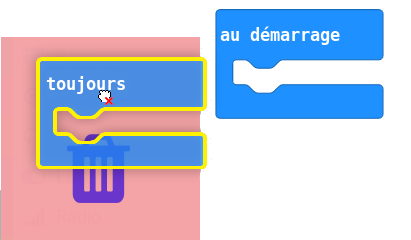
\includegraphics[scale=0.3]{res/mb-makecode_1erProg_suppr.png}
  \end{center}
\end{minipage}

\newpage

\begin{minipage}[t]{0.75\linewidth}
Pour construire le programme, il suffira par la suite de sélectionner les blocs adéquats parmi les catégories et de les enclencher pour créer des séquences d'instructions.
\end{minipage}
%   petit "ressort"
%   pour centrer les 2 colonnes
\hfill
%   colonne de droite
\begin{minipage}[t]{0.25\linewidth}~\\
  \vspace{-2mm}
  \begin{center}
    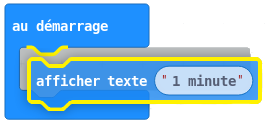
\includegraphics[scale=0.4]{res/mb-makecode_1erProg_enclencher2.png}
  \end{center}
\end{minipage}

\subsubsection{Définition du programme}

Nous voulons programmer un \mb qui :

\begin{itemize}

  \item allume toutes les LED lorsqu'on le secoue;
  \item éteigne les LED une par une à intervalle régulier;
  \item éteigne toutes les LED en 1 minute \mb.

\end{itemize}

Nous allons trouver les blocs nécessaires dans les catégories suivantes :

\begin{description}
  \item 
\includegraphics[width=8em]{res/blocsMkCd/MB_makecode_cat-base.png} Pour l'initialisation et l'affichage.
  \item 
\includegraphics[width=8em]{res/blocsMkCd/MB_makecode_cat-entrees.png} Pour l'interaction avec les boutons.
  \item 
\includegraphics[width=8em]{res/blocsMkCd/MB_makecode_cat-LED.png} Pour interagir avec chaque LED.
  \item 
\includegraphics[width=8em]{res/blocsMkCd/MB_makecode_cat-boucles.png} Pour répéter des instructions.
  \item 
\includegraphics[width=8em]{res/blocsMkCd/MB_makecode_cat-variables.png} Pour repérer les LED.
\end{description}



\subsubsection{Création du programme}


Voilà une proposition de programme pour réaliser notre objet :
\begin{center}
  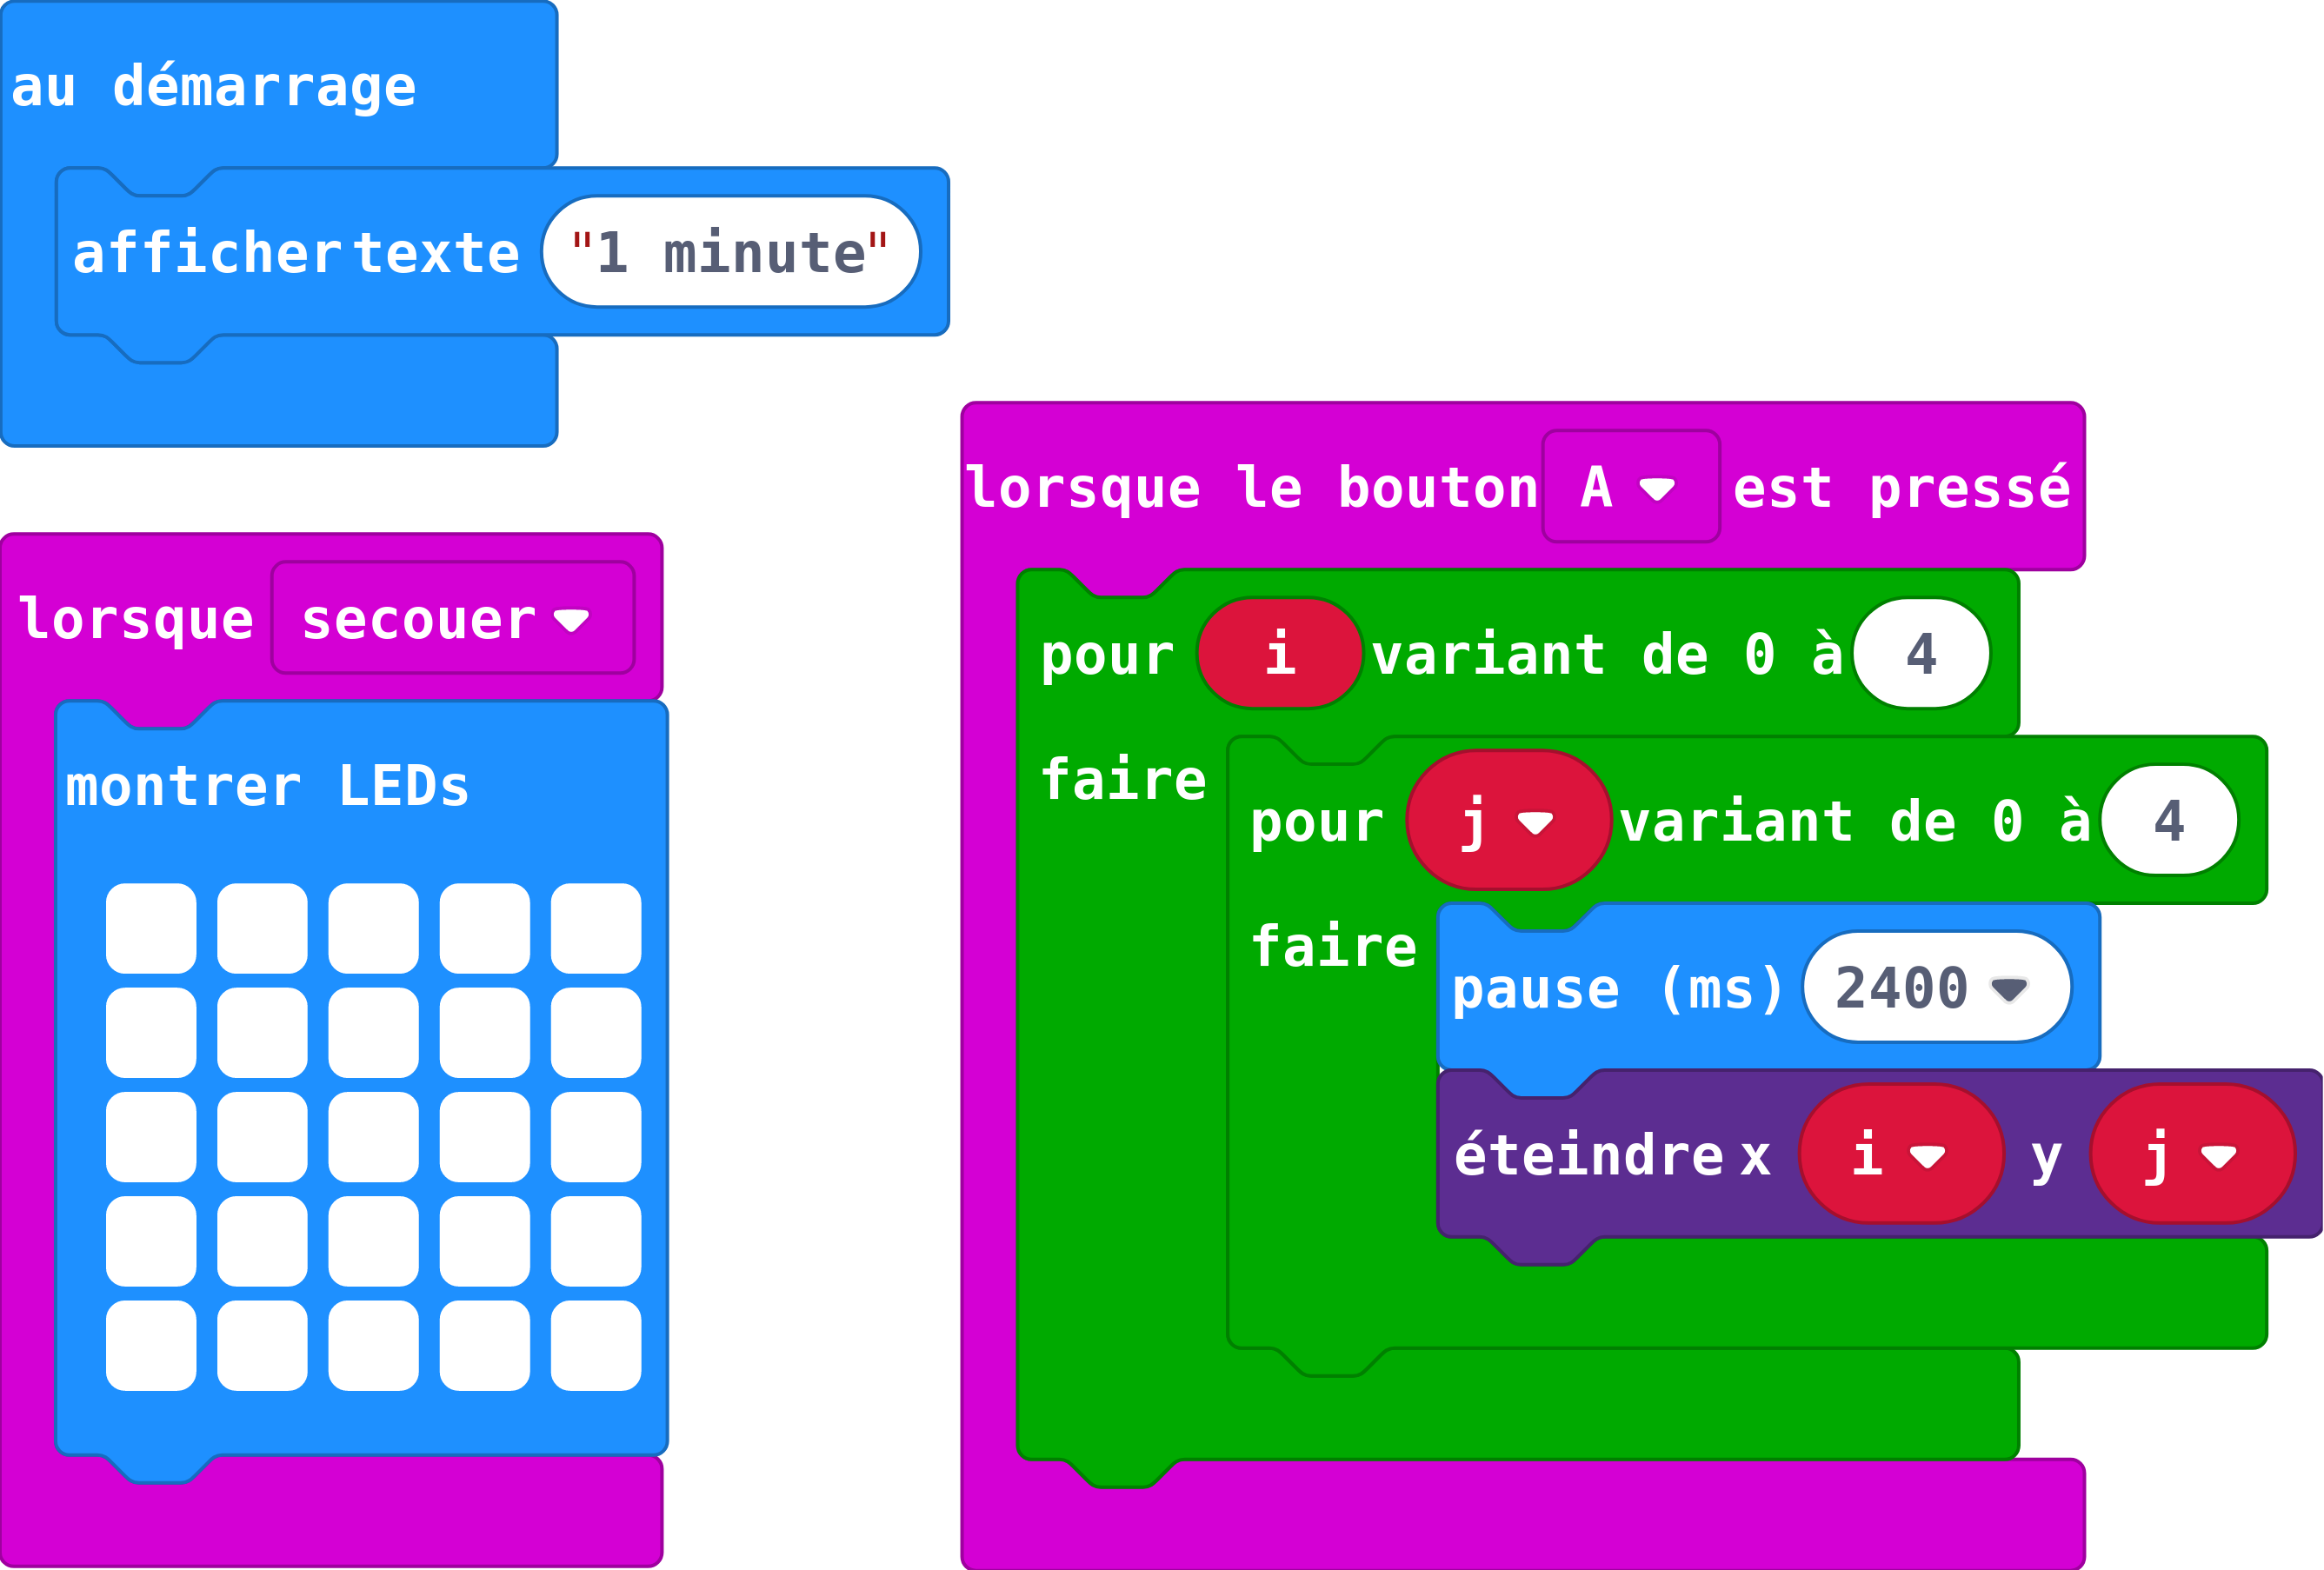
\includegraphics[width=0.6\linewidth]{res/mb-makecode_1erProg_eleve.png}
\end{center}

Il ne vous reste plus qu'à le télécharger. Le fichier sera compilé sous le nom microbit-XXXXX.hex et se retrouvera sur votre ordinateur dans votre dossier des téléchargements.\\
Pour flasher le \mb avec, il suffit de déplacer ce fichier vers la carte, qui doit être reconnue comme un lecteur USB par votre gestionnaire de fichiers.


\begin{remarque}


\includegraphics[width=0.2\linewidth]{res/mb-makecode_BtnAppairer.png}

Si vous utilisez le navigateur Chrome \textregistered, il est possible d'appairer le \mb (protocole webUSB) afin de téléverser le code directement sur la carte ce qui évite d'avoir à télécharger le fichier compilé puis à le copier manuellement.
\end{remarque}


\subsubsection{Explication du programme}

\begin{minipage}[t]{0.75\linewidth}

Dans ce programme, la principale difficulté consiste à éteindre les LED une par une.

Il faut savoir que les LED sont repérées par leur abscisse (x) et leur ordonnée (y).

La LED de coordonnées (0,0) est située en haut à gauche et la LED de coordonnées (4,4) est située en bas à droite.
\end{minipage}
%   petit "ressort"
%   pour centrer les 2 colonnes
\hfill
%   colonne de droite
\begin{minipage}[t]{0.25\linewidth}~\\
  \vspace{-2mm}
  \begin{center}
    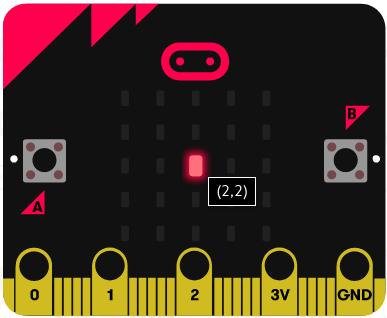
\includegraphics[scale=0.3]{res/mb-makecode_reperageLED.png}
  \end{center}
\end{minipage}


Nous allons donc utiliser ces paramètres dans des boucles "\emph{pour}" imbriquées. Une boucle va parcourir les valeurs de \textit{x}, et l'autre les valeurs de \textit{y}.


\begin{minipage}[t]{0.75\linewidth}

La boucle "\emph{pour}" utilise une variable (par exemple "\emph{i}" ou "\emph{index}") qui est créée automatiquement lorsqu'on utilise ce bloc.
\end{minipage}
%   petit "ressort"
%   pour centrer les 2 colonnes
\hfill
%   colonne de droite
\begin{minipage}[t]{0.25\linewidth}~\\
  \vspace{-2mm}
  \begin{center}
    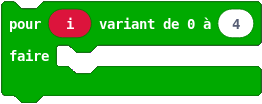
\includegraphics[scale=0.4]{res/blocsMkCd/MB_makecode_boucles-parcourir.png}
  \end{center}
\end{minipage}



\begin{minipage}[t]{0.75\linewidth}
Nous avons besoin de deux variables : une pour les valeurs de \textit{x}, l'autre pour les valeurs de \textit{y}.

Il faudra donc en créer une nouvelle (par exemple "\emph{j}") pour parcourir les valeurs de \textit{y}.
\end{minipage}
%   petit "ressort"
%   pour centrer les 2 colonnes
\hfill
%   colonne de droite
\begin{minipage}[t]{0.25\linewidth}~\\
  \vspace{-2mm}
  \begin{center}
    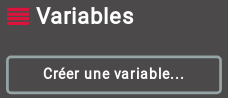
\includegraphics[scale=0.5]{res/mb-makecode_creer_variable.png}
  \end{center}
\end{minipage}


Puisque la durée est fixée à 1 minutes, c'est à dire 60 000 millisecondes et qu'il y a 25 LED, avant chaque extinction de LED il faut faire une pause d'une durée de $\frac{60 000}{25} = 2400$ millisecondes.
